\section{엔진 런타임 검증 및 실증 결과}\label{sec:eval}
본 절은 실시간 게임 엔진 보증에 초점을 맞춘 비혼합 2계층 평가를 제시한다: (i)~유한 권한 그래프, 헤드리스 Godot~4.7.1 장기 실행, 다중 엔진 프레임 예산 벤치마크 및 Datalog 스케일링을 다루는 0-LLM 결정론적 검증과, (ii)~직접 HTTPS Anthropic Claude~5.5 API 인증 스위트(\textbf{P15}--\textbf{P17}: Haiku·Sonnet·Opus~5.5 총 2.25M 토큰, deprecated \texttt{temperature} 생략 및 \texttt{output\_config.json\_schema} 적용) 및 3모델군 CLI(\textbf{P11}--\textbf{P14}, 실패 전량 보존)이다. 미실행 코호트(전향적 파일럿 0/180 \texttt{20261103}은 \texttt{NOT\_RUN/BLOCKED}로 기록, 인간 플레이테스트 \texttt{TR01--TR06} $N{=}0$은 \texttt{AWAITING\_HUMAN\_RATERS}로 명시)는 시스템/엔지니어링 트랙 검증 범위에 따라 머신 텔레메트리로부터 엄격히 분리한다.

\subsection{결정론적 게이트 한계, 권한 경계 및 Datalog 스케일링}\label{sec:tog-det}
신경망 정책 연결 전 버전 관리 엔진 브리지(\texttt{game-track/godot/scripts/sealed\_\allowbreak lighthouse\_\allowbreak machine.gd} 및 최대 8방·3역할 5월드)를 검증하였다. 1,664건 유한 그래프 감사(팔당 416건$\times$4 + 표면 감시 48건)에서 \texttt{schema\_only}는 260/416건의 유효하지 않은 제안을 커밋한 반면, 의미 게이트는 \textbf{0/416} 위험 커밋, 0/156 오거부, 128/260건 $\rho$ 수리(목표 252/416 대 124/416)를 달성했다. 확장 0-LLM 감사에서는 다중 오류 유계 수렴(\textbf{A1}: 위험 0/1,408, 충돌 동결 128/128), 서브밀리초 검증 지연(\textbf{A2}: $N{=}2000$ p95 0.0042--0.0751\,ms, $R{=}256$ 폐쇄 0.312--0.478\,ms), 주입 결함 추적성(\textbf{A3}: 4,656/4,656) 및 헤드리스 Godot~4.7.1 장기 실행(\textbf{A4}: 거부 코드 9/9 전량 실행, 상태 격리 11/11, 200에피소드 1,600/1,600틱 일관성, \texttt{step\_commit} p95 지연 \textbf{0.708\,ms}[60\,Hz 16.6\,ms 프레임 예산 이내], 정적 메모리 델타 $-268$\,B, 상태 누출 0건; 그림~\ref{fig:engine-cutscenes})을 확인하였다. 절차적 Datalog 스케일링(\textbf{P9}, $R\in\{8..64\} \times d\in\{1..5\}$ 480건; 표~\ref{tab:tog-datalog})에서 \texttt{nesy\_game.multihop}은 $\le$7.12\,$\mu$s의 중앙값 지연으로 100.0\% [99.21\%, 100.0\%] 상향식 오라클 일치를 달성한 반면, 평면 1홉은 46.67\%, 유계 2홉은 60.00\%에 그쳤다($Q{=}1100.19$).

\begin{figure*}[!tbp]
\centering
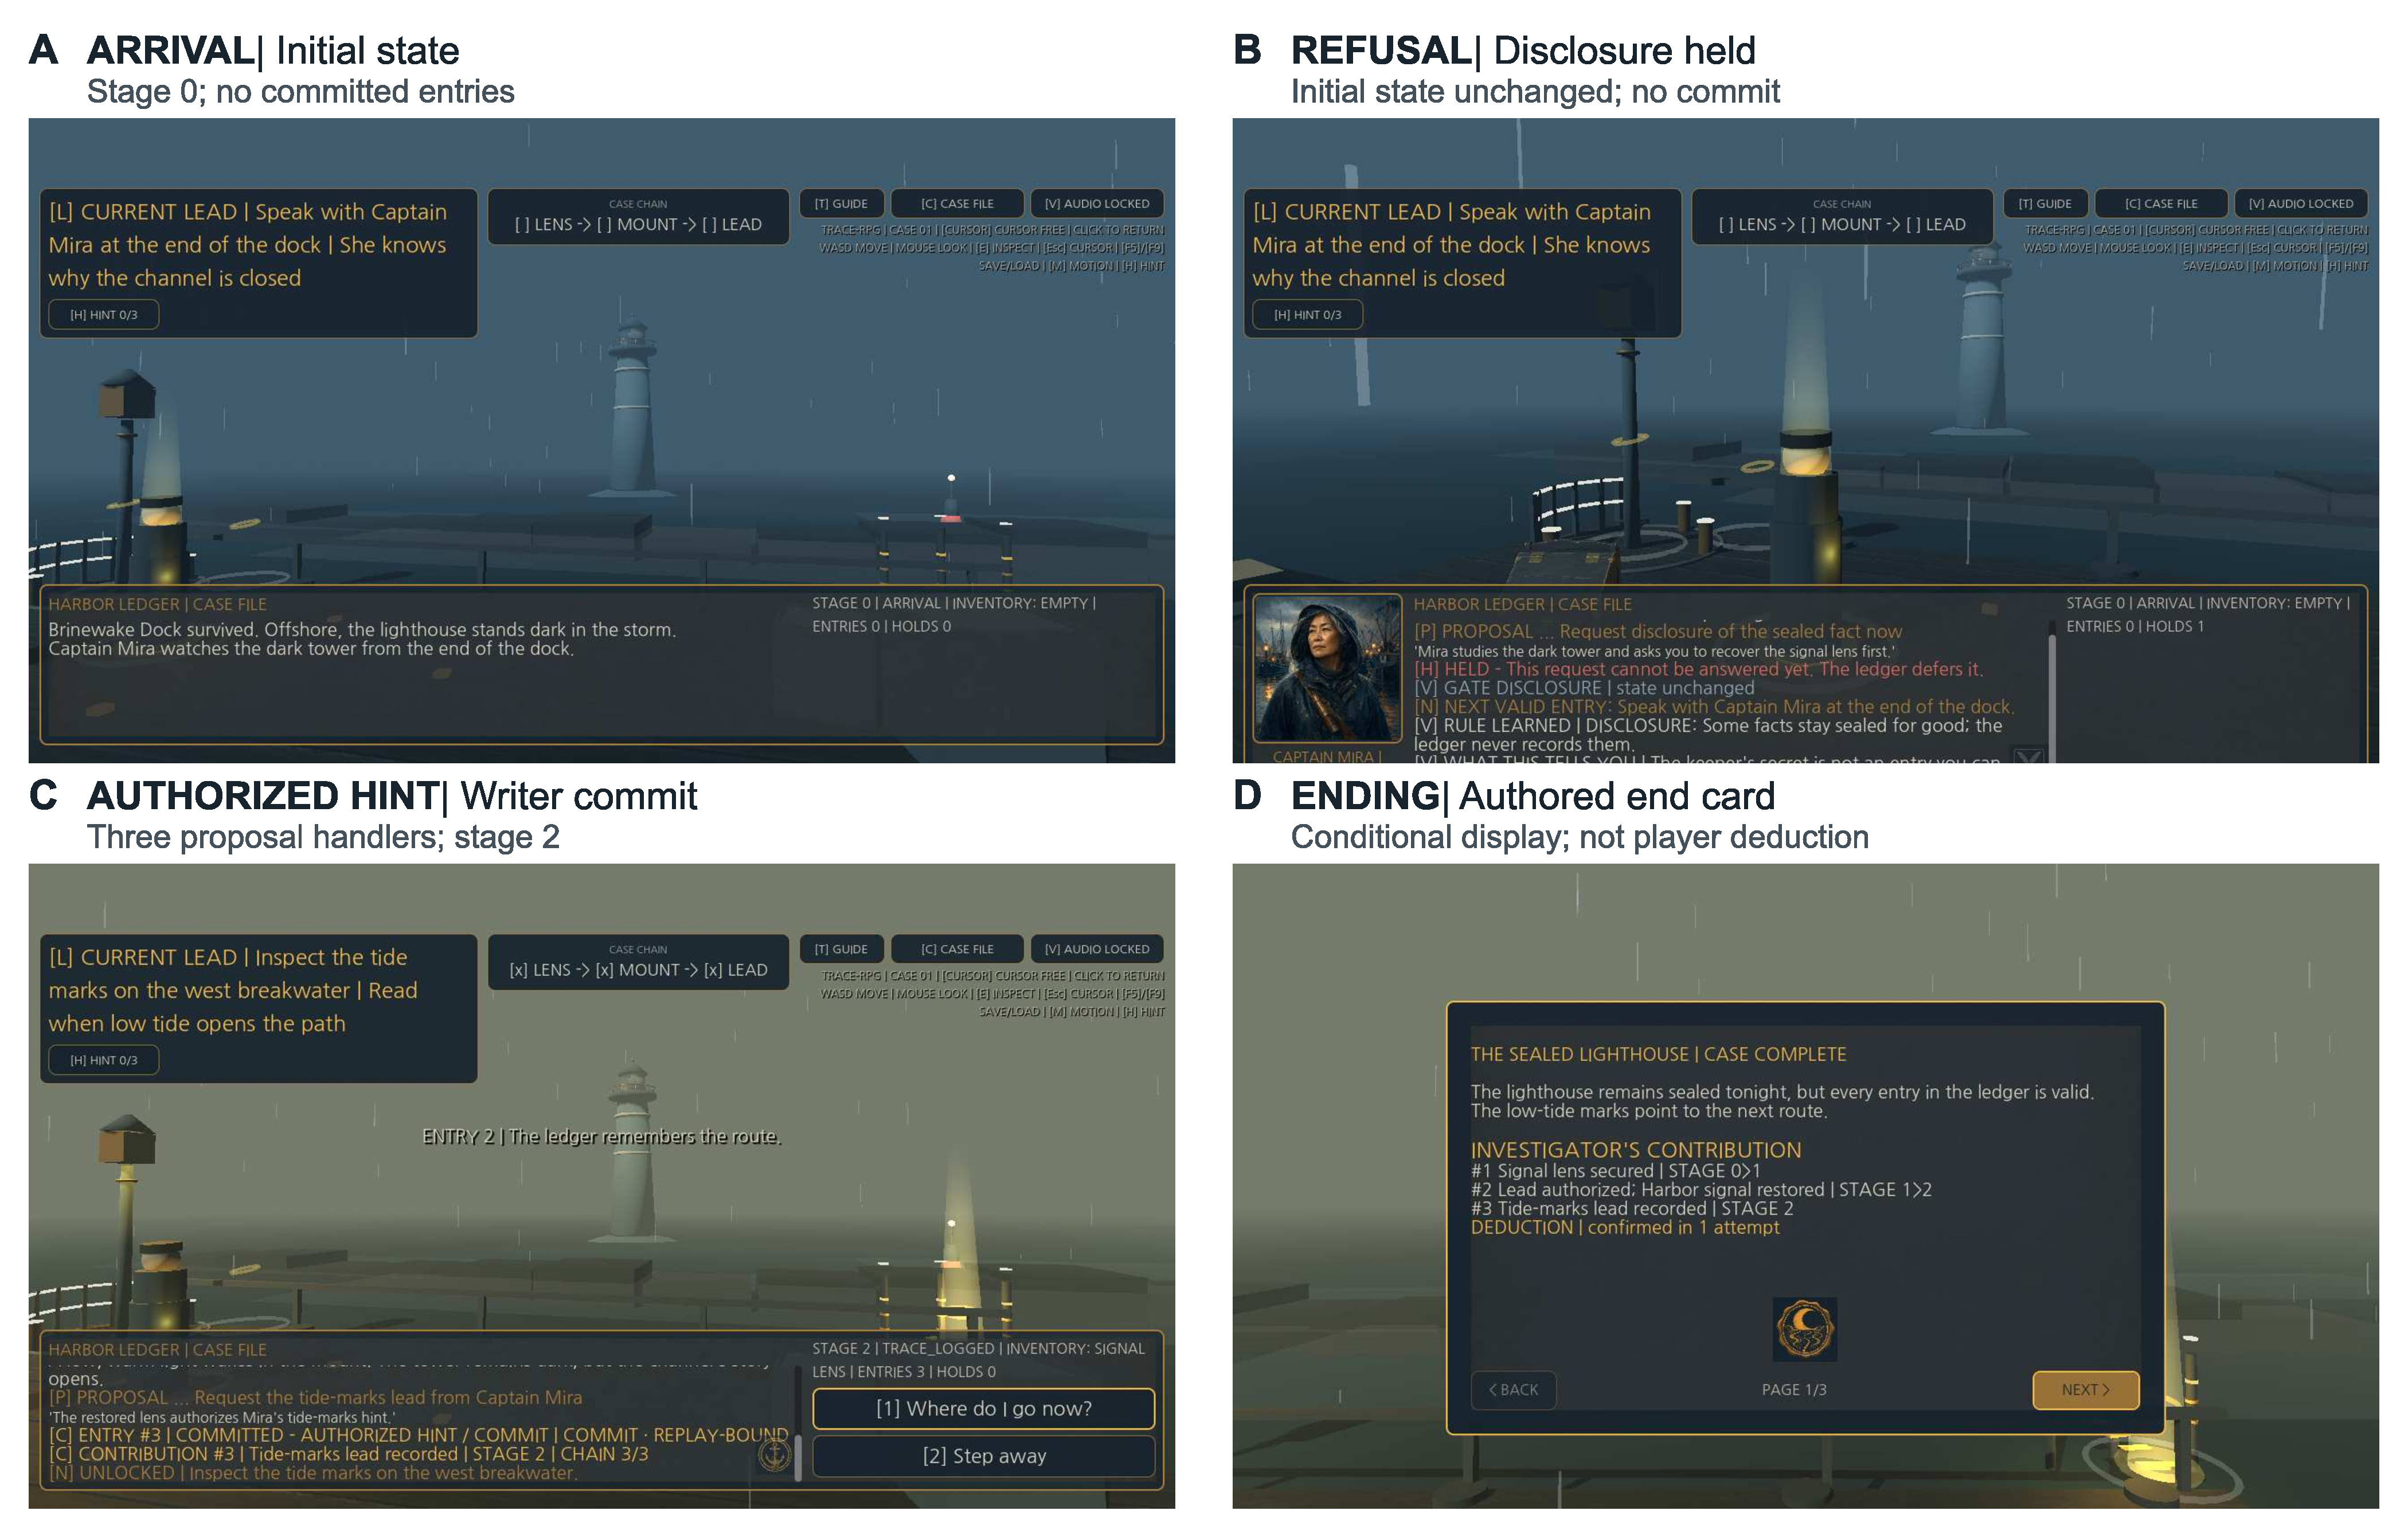
\includegraphics[width=0.90\textwidth]{../../figures/fig_engine_cutscenes.pdf}
\caption{네이티브 Godot~4.7.1 엔진 상태 머신 캡처: (A)~초기 도착, (B)~정본 상태 불변 비밀 공개 거부, (C)~2단계 인가 힌트, (D)~조건부 종료 카드.}
\Description{네이티브 Godot 4.7.1 4분할 스크린샷: 초기 도착, 비밀 공개 거부, 2단계 힌트, 조건부 종료 화면.}
\label{fig:engine-cutscenes}
\end{figure*}

\begin{table}[!tbp]
\caption{엔진 게이트 지연 및 다중 홉 오라클 스케일링 (\textbf{P9}: 480건, 0-LLM)}
\label{tab:tog-datalog}
\centering
\scriptsize
\setlength{\tabcolsep}{3pt}
\begin{tabularx}{\columnwidth}{@{}lcccc@{}}
\toprule
\textbf{검증기 구성} & \textbf{정확도 (480)} & \textbf{누출} & \textbf{중앙값 ($\mu$s)} & \textbf{p95 ($\mu$s)} \\
\midrule
\texttt{schema\_only} / \texttt{affordance} & 16.67\% (80) & 400 & --- & --- \\
\texttt{flat\_1hop\_gate} & 46.67\% (224) & 256 & 0.87--1.57 & 1.37--2.18 \\
\texttt{bounded\_2hop\_gate} & 60.00\% (288) & 192 & 1.88--2.58 & 2.66--3.91 \\
\texttt{nesy\_game.multihop} & \textbf{100.0\% (480)} & \textbf{0} & \textbf{6.46--7.12} & 9.83--11.42 \\
\bottomrule
\end{tabularx}
\end{table}

\subsection{네이티브 Godot~4.7.1 런타임 동등성 및 다계층 장기 실행 (\textbf{P19A} 및 \textbf{P19B})}\label{sec:tog-p19}
형식적 Python 참조 의미론이 네이티브 인터랙티브 게임 환경으로 정확히 전달되는지 보증하기 위해, 공식 헤드리스 Godot~4.7.1(\texttt{4.7.1.stable.official.a13da4feb}) 런타임 검증을 수행하였다. 모든 실행은 제품 저장소(\texttt{game-track/godot/})를 변경하지 않는 임시 프로젝트 샌드박스에서 수행되었다.

\textbf{교차 런타임 동등성 (\textbf{P19A}):} 표~\ref{tab:p19a-parity}에 나타난 바와 같이, 5개 상징적 퀘스트 그래프(\texttt{sealed-lighthouse-v1}, \texttt{sunken-archive-v1}, \texttt{clockwork-observatory-v1}, \texttt{ivory-citadel-v1}, \texttt{glass-foundry-v1}) 전반에서 120건의 전체 테스트(월드당 24건)를 평가하였다. 그 결과 \textbf{Python--Godot 상태 불일치 0건}, \textbf{Godot--오라클 논리 불일치 0건}, \textbf{신규 프로세스 재실행 불일치 0건}을 기록하였다. 네이티브 GDScript에서 엔진 상태 머신 검증은 p50 \textbf{5.0\,$\mu$s}, p95 \textbf{8.0\,$\mu$s}의 초고속 지연으로 완료된다. 아울러 5개 월드 에피소드 전체의 최종 상태는 독립 신규 프로세스의 터미널 SHA-256 해시와 정확히 일치하였으며, \textbf{0건의 위험 커밋}과 \textbf{0건의 비밀 누출}을 유지하였다.

\begin{table}[!tbp]
\caption{공식 헤드리스 Godot~4.7.1 교차 런타임 동등성 (\textbf{P19A}: 5개 상징적 월드 120건, 0-LLM)}
\label{tab:p19a-parity}
\centering
\scriptsize
\setlength{\tabcolsep}{2.5pt}
\begin{tabularx}{\columnwidth}{@{}>{\raggedright\arraybackslash}Xccccc@{}}
\toprule
\textbf{상징적 월드 그래프} & \textbf{건수} & \textbf{Py--GD} & \textbf{오라클} & \textbf{GD 지연시간} & \textbf{SHA-256} \\
\midrule
\texttt{sealed-lighthouse-v1}     & 24/24 & 0 & 0 & 5.0\,$\mu$s / 8.0\,$\mu$s & 일치 (0누출) \\
\texttt{sunken-archive-v1}        & 24/24 & 0 & 0 & 5.0\,$\mu$s / 8.0\,$\mu$s & 일치 (0누출) \\
\texttt{clockwork-obs-v1}         & 24/24 & 0 & 0 & 5.0\,$\mu$s / 8.0\,$\mu$s & 일치 (0누출) \\
\texttt{ivory-citadel-v1}         & 24/24 & 0 & 0 & 5.0\,$\mu$s / 8.0\,$\mu$s & 일치 (0누출) \\
\texttt{glass-foundry-v1}         & 24/24 & 0 & 0 & 5.0\,$\mu$s / 8.0\,$\mu$s & 일치 (0누출) \\
\midrule
\textbf{전체 / 집계 동등성} & \textbf{120/120} & \textbf{0} & \textbf{0} & \textbf{5.0\,$\mu$s / 8.0\,$\mu$s} & \textbf{5/5 (0위험)} \\
\bottomrule
\end{tabularx}
\end{table}

\textbf{대규모 다계층 엔진 장기 실행 (\textbf{P19B}):} 지속적인 상태 변이 부하 하에서의 엔진 안정성을 검증하기 위해, 5개 구조적 복잡도 계층($R\in\{8..128\}$, 행동 알파벳 $A\in\{3..16\}$, 의존 깊이 $d\in\{2..8\}$; 표~\ref{tab:p19b-soak})에 걸쳐 5,000틱 장기 실행 시험을 실시하였다. 5,000틱 동안 시스템은 3,750건의 인가된 커밋을 성공적으로 처리하고, 1,250건의 결정론적 $\rho$ 반례 수리를 발동시켰으며, 1,875건의 적대적 비밀 누출 시도를 안전하게 차단하였다. 특히 엔진 상태에는 \textbf{단 1건의 위험 커밋이나 비밀 누출도 발생하지 않았으며}(\textbf{0건}), 5/5 전 계층에서 신규 프로세스 터미널 SHA-256 해시가 완벽히 재현되었다. 가장 복잡한 Tier~5($R{=}128, A{=}16, d{=}8$)에서도 GDScript 검증 지연은 p50 0.017\,ms, p95 0.033\,ms, 최악 최대 지연 \textbf{0.074\,ms}에 불과하였다. 이는 60\,Hz 프레임 예산(16.667\,ms)의 \textbf{0.44\%}, 120\,Hz 프레임 예산(8.333\,ms)의 \textbf{0.89\%}만을 소비하는 것으로, \textbf{100\%의 프레임 예산 준수율}을 입증한다.

\begin{table}[!tbp]
\caption{Godot~4.7.1 다계층 스케일링 및 프레임 예산 장기 실행 (\textbf{P19B}: 5,000틱, 3,750커밋, 1,250 $\rho$수리)}
\label{tab:p19b-soak}
\centering
\scriptsize
\setlength{\tabcolsep}{2.2pt}
\begin{tabularx}{\columnwidth}{@{}>{\raggedright\arraybackslash}Xcccccc@{}}
\toprule
\textbf{계층} & \textbf{그래프 구성} & \textbf{p50} & \textbf{p95} & \textbf{p99} & \textbf{최대} & \textbf{60/120\,Hz} \\
\midrule
Tier 1 & $R{=}8, A{=}3, d{=}2$    & 0.011\,ms & 0.022\,ms & 0.022\,ms & 0.023\,ms & 0.14\% / 0.28\% \\
Tier 2 & $R{=}16, A{=}4, d{=}3$   & 0.012\,ms & 0.024\,ms & 0.024\,ms & 0.027\,ms & 0.16\% / 0.32\% \\
Tier 3 & $R{=}32, A{=}8, d{=}5$   & 0.013\,ms & 0.027\,ms & 0.027\,ms & 0.037\,ms & 0.22\% / 0.44\% \\
Tier 4 & $R{=}64, A{=}12, d{=}6$  & 0.014\,ms & 0.029\,ms & 0.030\,ms & 0.059\,ms & 0.35\% / 0.71\% \\
Tier 5 & $R{=}128, A{=}16, d{=}8$ & 0.017\,ms & 0.033\,ms & 0.035\,ms & 0.074\,ms & 0.44\% / 0.89\% \\
\bottomrule
\end{tabularx}
\end{table}

\subsection{교차 엔진 프레임 예산 벤치마크 (\textbf{P18B})}\label{sec:tog-p18b}
실시간 게임 루프에서 논리 검증은 엄격한 프레임 데드라인 내에 완료되어야 한다. \textbf{P18B}에서는 1,080건의 절차적 게임 인스턴스($R \le 256, d \le 10$)를 바탕으로 \system{}를 최신 범용 기호 추론기들과 비교하였다. 네이티브 Godot GDScript 및 Python \texttt{nesy\_game}을 Clingo~5.8.3 답집합 프로그래밍(ASP) 해석기~\cite{gebser2019clingo}, Z3~5.4.1.0 SMT 해석기~\cite{demoura2008z3}, W3C OWL~2 RL 기술 논리 추론~\cite{motik2012owl2profiles}과 비교 검증하였다.

표~\ref{tab:cross-engine}에 요약된 바와 같이, $R{=}128$에서 네이티브 Godot GDScript 검증은 p50 0.017\,ms(60/120\,Hz 100\% 통과), Python \texttt{nesy\_game}은 0.179\,ms(100\% 통과)를 기록했다. Clingo~5.8.3 멀티샷 ASP는 3.017\,ms로 60\,Hz 및 120\,Hz 프레임 제한을 충족하였다. 반면 Z3~5.4.1.0 SMT는 p50 17.447\,ms의 지연시간을 보여 60\,Hz 데드라인을 11.67\%만 충족했고 120\,Hz는 0\%였다($R{=}256$에서는 p50 34.670\,ms로 60\,Hz 충족률 0\%). 규칙 기반 OWL~2 RL은 $R{=}64$에서 19,696\,ms가 소요되었고 $R \ge 128$에서는 20초 타임아웃을 초과하였다(프레임 충족률 0\%). 중요한 점은 4개 정밀 기호 시스템 모두 형식적 오라클 대비 \textbf{0건의 불일치}를 기록하여(Clingo 및 Z3 1,080/1,080건; OWL~2 RL 타임아웃 전 인증 165/165건) 정리~1의 건전성을 입증한 반면, 휴리스틱 평면 1홉 게이트(50.00\% 정확도) 및 유계 2홉 게이트(58.33\% 정확도)는 빈번히 실패했다(Cochran's $Q = 1948.24, p < 10^{-300}$). 이는 \system{}가 게임 엔진 프레임 레이트에서 산업용 솔버 수준의 건전성을 달성함을 입증한다.

\begin{table}[!tbp]
\caption{교차 엔진 프레임 예산 및 추론 벤치마크 (\textbf{P18B}: 1,080건 인스턴스, $R{\le}256, d{\le}10$, $R{=}128$ 평가)}
\label{tab:cross-engine}
\centering
\scriptsize
\setlength{\tabcolsep}{2.0pt}
\begin{tabularx}{\columnwidth}{@{}>{\raggedright\arraybackslash}Xccccc@{}}
\toprule
\textbf{엔진 / 정식화} & \textbf{p50} & \textbf{60\,Hz} & \textbf{120\,Hz} & \textbf{정확도 (1,080)} & \textbf{불일치} \\
\midrule
Godot GDScript (네이티브)              & \textbf{0.017\,ms} & \textbf{100\%} & \textbf{100\%} & \textbf{100.0\%} & \textbf{0} \\
Python \texttt{nesy\_game}             & 0.179\,ms & 100\% & 100\% & 100.0\% & 0 \\
Clingo 5.8.3 ASP~\cite{gebser2019clingo}  & 3.017\,ms & 100\% & 100\% & 100.0\% & 0 \\
Z3 5.4.1.0 SMT~\cite{demoura2008z3}       & 17.447\,ms & 11.7\% & 0.0\% & 100.0\% & 0 \\
OWL 2 RL~\cite{motik2012owl2profiles}     & $>$20\,s  & 0.0\% & 0.0\% & 100.0\%$^\dagger$ & 0 \\
\midrule
평면 1홉 게이트 (불완전)               & 0.001\,ms & 100\% & 100\% & 50.00\% & 540 \\
유계 2홉 게이트                        & 0.002\,ms & 100\% & 100\% & 58.33\% & 450 \\
\bottomrule
\end{tabularx}
\end{table}

\subsection{라이브 Godot~4.7.1 폐루프 엔진 리플레이 (\textbf{P16B} 및 \textbf{P13})}\label{sec:tog-godot}
표~\ref{tab:tog-godot}는 인증 API(\textbf{P16B}: Haiku·Sonnet·Opus~5.5 21에피소드, 169,071토큰) 및 3모델군 CLI(\textbf{P13}: 42에피소드)의 Godot~4.7.1(\texttt{4.7.1.\allowbreak stable.\allowbreak official.\allowbreak a13da4feb}) 종단간 실행을 정리한다. 전량 \textbf{21/21} API 및 \textbf{42/42} CLI 에피소드가 0-LLM 헤드리스 Godot 재실행을 100\% 통과하며 위험 커밋·비밀 유출이 \textbf{0/63}이었다. 실제 제품 \texttt{SealedLighthouseMachine}에서도 API \textbf{6/6 (100\%)} 전량이 \texttt{EXACT\_\allowbreak TERMINAL\_\allowbreak HASH}(\texttt{4b231017...})에 도달했다(Godot 251.64--1009.78\,ms 대 API 9.1--40.9\,s).

\begin{table}[!tbp]
\caption{헤드리스 Godot~4.7.1 폐루프 리플레이 및 지연 분해 (\textbf{P16B} 21 API + \textbf{P13} 42 CLI)}
\label{tab:tog-godot}
\centering
\scriptsize
\setlength{\tabcolsep}{2.2pt}
\begin{tabularx}{\columnwidth}{@{}>{\raggedright\arraybackslash}X*{5}{c}@{}}
\toprule
\textbf{Godot 트랙 / 모델 계층} & \textbf{목표} & \textbf{리플레이} & \textbf{누출} & \textbf{GD (ms)} & \textbf{API (s)} \\
\midrule
\textbf{P16B} 5월드 Haiku~5.5 & 5/5 & 5/5 & \textbf{0/5} & 757--1010 & 10.6--20.9 \\
\textbf{P16B} 5월드 Sonnet~5.5 & 4/5 & 5/5 & \textbf{0/5} & 252--1005 & 14.5--36.0 \\
\textbf{P16B} 5월드 Opus~5.5 & 4/5 & 5/5 & \textbf{0/5} & 253--1009 & 16.2--40.9 \\
\textbf{P16B} 제품 \texttt{SealedLighthouse} (6) & \textbf{6/6} (해시) & 6/6 & \textbf{0/6} & 751--779 & 9.1--16.5 \\
\textbf{P13} 3모델군 5월드 (30) & 23/30 & 30/30 & \textbf{0/30} & --- & CLI \\
\textbf{P13} 3모델군 제품 \texttt{Sealed} (12) & 9/12 (해시) & 12/12 & \textbf{0/12} & --- & CLI \\
\bottomrule
\end{tabularx}
\end{table}

\subsection{폐루프 다중 에이전트 실딩 및 요인 절단 (\textbf{P15}, \textbf{P16A}, \textbf{P12})}\label{sec:tog-mas}
\textbf{P15}(Haiku·Sonnet·Opus~5.5$\times$5월드$\times$7암 105에피소드, 1,048,803토큰, \textbf{105/105} 리플레이; 표~\ref{tab:kbs-mas})에서 Safe-RL 프록시~\cite{alshiekh2018shield}(목표 0/15, 위험 16/61)와 NeMo 프록시~\cite{rebedea2023nemo}(1/15, 15/61)는 다중 홉 누출을 놓쳤고, 평면 1홉도 3/15에피소드 4/66턴(\texttt{ivory-citadel-v1} 1에피소드 2턴, \texttt{glass-foundry-v1} 2에피소드 2턴)을 누출했다. 반면 \texttt{nesy\_game.multihop} 전 암은 \textbf{15/15 (100\%)} 무누출·\textbf{0} 위험을 유지했고, \texttt{rho\_k2}에서는 거부 18건 전부가 정리~2 상태 의존 거부여서 $\rho_{\mathrm{repairs}}{=}0$으로 무세탁을 실증했으며(14/15 대 13/15는 독립 1턴 표본 변동), 하이브리드 $\rho{+}\text{LLM}_{K=1}$은 20회 안전 재선정으로 \textbf{15/15 (100\%)} 목표를 달성했다($Q_{\mathrm{goal}}{=}68.71$). \textbf{P16A}(60에피소드, 673,869토큰)에서는 정책·단계 결함에 대해 $\rho$가 \textbf{22건 라이브 수리}(Haiku 18, Sonnet 4)를 실행해 30/30 무누출·11/30 목표를 달성했고(대조 \texttt{general\_rule} 22/30·9위험), \textbf{P12} 27결함 $(a,E)$ 수리도 $\rho_{K=2}$ \textbf{27/27}(0토큰) 대 LLM 26/27(530k--542k토큰, $p{=}1.0$)이었다.

\begin{table*}[!tbp]
\caption{인증 독립 폐루프 7-암 다중 에이전트 실딩 및 수리 분해 (\textbf{P15}: 105에피소드, 105/105 0-LLM 리플레이)}
\label{tab:kbs-mas}
\centering
\scriptsize
\setlength{\tabcolsep}{3.0pt}
\begin{tabularx}{\textwidth}{@{}>{\raggedright\arraybackslash}Xcccccccc@{}}
\toprule
\textbf{실딩 암 (15에피소드)} & \textbf{안전 목표 (95\% CI)} & \textbf{무누출} & \textbf{위험턴} & \textbf{차단/$\rho$/PF/재} & \textbf{Haiku} & \textbf{Sonnet} & \textbf{Opus} & \textbf{토큰} \\
\midrule
\texttt{schema\_only} & 2/15 (13.3\%) [3.7, 37.9] & 2/15 & 16/59 & 0 / 0 / 0 / 0 & 1/1/6 & 1/1/4 & 0/0/6 & 133,054 \\
\texttt{safe\_rl\_action\_mask}~\cite{alshiekh2018shield} & 0/15 (0.0\%) [0.0, 20.4] & 1/15 & 16/61 & 2 / 0 / 0 / 0 & 0/1/5 & 0/0/5 & 0/0/6 & 139,205 \\
\texttt{nemo\_colang\_rail}~\cite{rebedea2023nemo} & 1/15 (6.7\%) [1.2, 29.8] & 1/15 & 15/61 & 1 / 0 / 1 / 0 & 0/0/5 & 0/0/5 & 1/1/5 & 136,515 \\
\texttt{flat\_1hop\_shield} & 12/15 (80.0\%) [54.8, 93.0] & 12/15 & 4/66 & 15 / 0 / 0 / 0 & 4/4/1 & 5/5/0 & 3/3/3 & 146,446 \\
\texttt{multihop\_shield\_k0} & 13/15 (86.7\%) [62.1, 96.3] & \textbf{15/15} & \textbf{0/69} & 22 / 0 / 0 / 0 & 4/5/0 & 5/5/0 & 4/5/0 & 152,649 \\
\texttt{trace\_rpg\_multihop\_rho\_k2} & 14/15 (93.3\%) [70.2, 98.8] & \textbf{15/15} & \textbf{0/68} & 18 / 0 / 0 / 0 & 5/5/0 & 5/5/0 & 4/5/0 & 150,986 \\
\texttt{trace\_rpg\_hybrid\_rho\_llm\_k1} & \textbf{15/15 (100\%)} [79.6, 100] & \textbf{15/15} & \textbf{0/63} & 2 / 0 / 1 / 20 & \textbf{5/5/0} & \textbf{5/5/0} & \textbf{5/5/0} & 189,948 \\
\bottomrule
\end{tabularx}
\end{table*}

\subsection{양방향 의미론적 우회 강건성 (\textbf{P20} 및 \textbf{P17}) 및 엔지니어링 범위}\label{sec:tog-p20-scope}
\textbf{1,200건 양방향 의미론적 우회 (\textbf{P20}):} 적대적 에이전트는 언어적 난독화나 다국어 어휘 위장을 통해 게이트 실딩을 우회하려 시도할 수 있다. 힌트 없는 의미론적 우회에 대한 게이트 경계 탄력성을 검증하기 위해, \textbf{P20}에서는 6개 게임 서사 도메인 $\times$ 5개 의미 층위 $\times$ 한국어 및 영어 표현 $\times$ 셀당 20건으로 체계적으로 층화된 1,200건의 통제 사례를 평가하였다. 한·영 테스트 쌍 간의 어휘 Jaccard 유사도는 0.0630으로 엄격히 제한되어, 피상적 음역이 아닌 진정한 의미적 분기가 이루어졌음을 보증한다.

도메인 배제(LODO) 교차 검증에서 기본 구문 검사는 취약함을 드러냈다: \texttt{stage1\_id\_only}는 60.00\%의 정확도에 그쳤고, 단순 키워드 규칙(\texttt{keyword\_rule\_naive})은 62.67\% 정확도에 정상적인 Stage-4 서사 대화에서 98.33\%의 치명적인 오거부율(S4 FRR)을 기록했다. 반면 층화 n-그램 및 경계 분류기(\texttt{tfidf\_char\_word\_lodo})는 \textbf{97.17\% 정확도}와 단 \textbf{1.25\%의 S4 FRR}을 달성하였다. 비모수 검정은 필터링 전략 간의 유의미한 차이를 확증한다(Cochran's $Q = 871.39, df=4, p = 2.63 \times 10^{-187}$).

\textbf{통합 Stage-2 API 우회 검증 (\textbf{P17}):} 540건의 통합 프롬프트 한·영 Stage-2 우회 평가(\textbf{P17}: 180건 $\times$ 3계층, 단락 회로 0건, 359,030토큰, $\kappa{=}0.8813$, $Q{=}9.5$; 3모델군 \textbf{P14} $\kappa{=}0.9367$)에서 Claude~5.5는 \textbf{0/72 (0.0\%) FRR}에서 94.44--97.22\%의 패러프레이즈 재현율을 달성한 반면(Haiku $F_1{=}0.957$, Opus $0.925$, Sonnet $0.904$), 산문 내 힌트 없는 원시 ID는 놓쳐(19--29/36), Stage-1과 Stage-2의 상보성을 입증하였다.

\textbf{아카이빙 엔지니어링 트랙 범위 및 연구 윤리:} 본 논문은 결정론적 게임 엔진 런타임 검증, 형식적 온톨로지 실딩, 결정론적 리플레이 아키텍처를 다루는 시스템 및 소프트웨어 공학 연구로 명시적 범위를 한정한다. 기계 런타임 검증과 주관적 플레이어 경험은 다음과 같이 엄격히 분리된다:
\begin{enumerate}
    \item 인간 플레이테스트 코호트($N{=}0$, \texttt{TR01--TR06})는 \texttt{AWAITING\_HUMAN\_RATERS}로 엄격히 유지된다. 시뮬레이션되거나 추측된 플레이어 인지 점수로 대체하지 않는다.
    \item 전향적 플레이어 파일럿 연구(0/180, \texttt{20261103})는 \texttt{NOT\_RUN/BLOCKED}로 기록되며 기계 텔레메트리로부터 엄격히 격리된다.
    \item 오픈 사이언스 아티팩트와 스키마는 \texttt{DATASHEET\_v5.md}~\cite{gebru2021datasheets} 및 Croissant~1.0 v5~\cite{akhtar2024croissant}로 체계적으로 문서화된다.
\end{enumerate}
